\documentclass[a4paper, 10pt]{article}
\usepackage[utf8]{inputenc} % Change according your file encoding
\usepackage{graphicx}
\usepackage{url}
\usepackage{amsmath}
\usepackage{mathtools}
\usepackage{mathrsfs}
\usepackage{amsfonts}
\usepackage{bbm}
\usepackage{amsthm}
\usepackage{amssymb}
\usepackage{fancyhdr}
\usepackage{setspace}
\usepackage{tabularx}
\usepackage{tcolorbox}
\usepackage{tikz}
\usepackage[a4paper, left=2cm, right=2cm, top=2.5cm, bottom=2cm]{geometry}
\usepackage[ruled]{algorithm2e}

% Links, link colors, and clickable ToC
\usepackage{hyperref}
\hypersetup{
    colorlinks,
    citecolor=black,
    filecolor=black,
    linkcolor=black,
    urlcolor=black
}

\pagestyle{fancy}
\fancyhf{}
\rhead{Group 2 - Problem \thesection}
\lhead{M. Altarriba, E. Gonzalvo, A. Mir, C. Segarra}
\cfoot{\thepage}

% New commands
\newcommand{\Z}{\mathbb{Z}}
\newcommand{\F}{\mathbb{F}}
\newcommand\tab[1][1cm]{\hspace*{#1}}
\renewcommand{\P}{\mathcal{P}}

\newtheorem{obs}{Observation}
\newtheorem{theorem}{Theorem}
\newtheorem*{theoremstar}{Theorem}

\theoremstyle{definition} % amsthm only
\newtheorem{definition}{Definition}

\begin{document}
\onehalfspacing
\pagestyle{empty}

\begin{center}
    \vspace{2cm}
    
\includegraphics[width=8cm]{img/logo_fme.png}
    \vspace{2cm}

    \Large
    Master in Advanced Mathematics and Mathematical Engineering
    \vspace{0.5cm}

    \LARGE
    Codes \& Cryptography: Problem Assignment - Group 2

    \vspace{0.5cm}
    \large
    Marta Altarriba, Eduard Gonzalvo, Arnau Mir, Carlos Segarra

    \vspace{0.5cm}
    \normalsize
    \today

    \vspace{1cm}

\end{center}

\tableofcontents


\newpage
\pagestyle{fancy}
\section{Problem 1: Secure PRP}\label{sec:problem1}

Suppose $F$ is a secure PRP with blocklength $\lambda$.
Give the decryption algorithm for the following scheme and prove that it does not have CPA security:

\begin{figure}[h!]
    \centering
\begin{minipage}[t]{.45\textwidth}
\null 
 \begin{algorithm}[H]
    \DontPrintSemicolon
    $\mathcal{K} \gets \{\textcolor{red}{0}, \textcolor{red}{1}\}^{\lambda}$ \;
    $\mathcal{M} \gets \{ \textcolor{red}{0} , \textcolor{red}{1} \}^{2\lambda}$ \;
    $\mathcal{C} \gets \left( \{ \textcolor{red}{0} , \textcolor{red}{1} \}^{\lambda}\right)^3$ \;
    \Begin{
        $k \gets \{ \textcolor{red}{0}, \textcolor{red}{1} \}^{\lambda} $ \;
        \KwRet{$k$}
    }
    \caption{Key generation procedure}
  \end{algorithm}
\end{minipage}%
\begin{minipage}[t]{.45\textwidth}
\null
 \begin{algorithm}[H]
    \DontPrintSemicolon
    \Begin{
        $r \gets \{ \textcolor{purple}{0} , \textcolor{purple}{1} \}^\lambda$ \;
        $s \gets F_k (r \oplus m_1)$ \;
        $t \gets F_k (r \oplus m_1 \oplus F_k (m_1) \oplus m_2)$ \;
        $c \gets \langle r$ $\vert \vert$ $s$ $\vert \vert$ $t \rangle$ \;
        \KwRet{$c$}
    }
     \vspace{4.4pt}
    \caption{Encryption algorithm}
  \end{algorithm}
\end{minipage}
    \caption{Encryption and key generation scheme for Problem 1.\label{prob1:encryption}}
\end{figure}
\begin{center}
    \rule{5cm}{0.4pt}
\end{center}

\textbf{\textit{Proof:}}
For the decryption algorithm, we will assume we are given the pseudo-random permutation F and its associated key $k$.
We also assume access to the cipher text, which consists of a concatenation of 3 parameters: $r$, $s$ and $t$.
Lastly, the plain text will be of the form $m = \langle m_1$ $\vert \vert$ $m_2 \rangle$.

To find each of its two parts we will isolate them from the $s$ and $t$ expressions.
This can be easily done as F is a secure PRP and, therefore, efficiently invertible.
Also, the $\oplus$ (XOR) operator can be inverted using the relation $a \oplus b = c \Leftrightarrow a = c \oplus b$.
The full decryption algorithm for the encryption scheme in Figure~\ref{prob1:encryption} is depicted in Algorithm~\ref{fig1:decryption}.
\begin{algorithm}
    \DontPrintSemicolon
    \KwData{Cipher text composed of three parameters - $r$, $s$, and $t$ - concatenated together.}
    \KwResult{Plain text $m$}
    \Begin{
        $m_1 \gets F_k^{-1} (s) \oplus r; \hspace{5pt}$\;
        $m_2 \gets F_k^{-1} (t) \oplus r \oplus m_1 \oplus F_k (m_1)$ \;
        $m \gets \langle m_1 \vert \vert m_2 \rangle $ \;
        \KwRet{$m$}
    }
    \caption{Decryption algorithm for the given scheme.\label{fig1:decryption}}
\end{algorithm}

To verify the correctness of the decryption algorithm, we can check that $Dec_k (Enc_k (m)) = m$, for every message $m \in \mathcal{M}$.

%Now, to show that this scheme is not CPA-secure, we need to put ourselves in the adversary's shoes. This means that we no longer have access to the PRP, nor the private key $k$, but we are able to know the ciphertext associated to a chosen plaintext, for various queries.

%One of the main techniques that witnesses a non CPA-secure scheme is to check that it is deterministic (not randomized). Clearly, this one is not the case, so we'll have to think it twice.
To prove that the scheme from Figure~\ref{prob1:encryption} is not CPA secure we will use the attack game depicted in Figure~\ref{prob1:attack-game}.

\begin{figure}[h!]
    \centering
    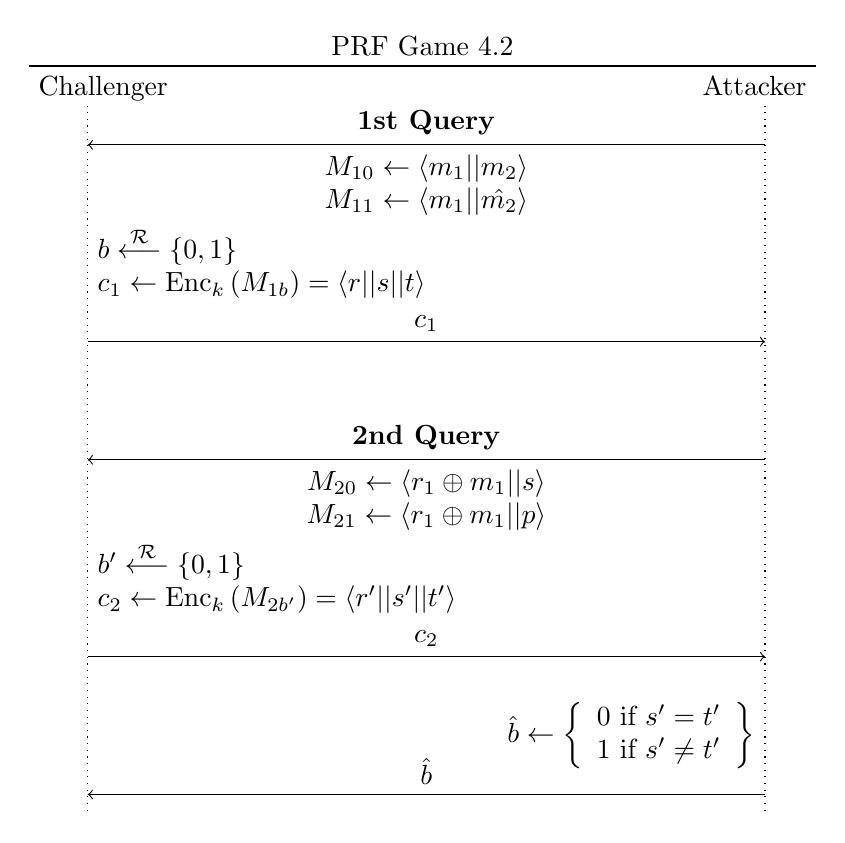
\begin{tikzpicture}
        % Define Variables
        \def\lR{0.75}
        \def\rR{9.35}
        \def\bottom{-9.5}

        % Overall Scheme
        \draw[thick] (0,0) -- (10,0) node[midway, anchor=south] {PRF Game $4.2$};
        \node[anchor = north west] at (0,0) (c-r) {Challenger};
        \draw[dotted] (\lR, -0.5) -- (\lR,\bottom);
        \node[anchor = north east] at (10,0) {Attacker};
        \draw[dotted] (\rR, -0.5) -- (\rR, \bottom);

        % 1st Query
        \draw[->] (\rR, -1) -- (\lR, -1) node[midway, anchor=south] {\textbf{1st Query}} node[midway, anchor=north, align=center] {$M_{10} \gets \langle m_1 \vert \vert m_2 \rangle$ \\ $M_{11} \gets \langle m_1 \vert \vert \hat{m_2} \rangle$};
        \node[anchor=west, align=left] at (\lR, -2.5) {$b \overset{\mathcal{R}}{\longleftarrow} \{0,1\}$ \\ $c_1 \gets \text{Enc}_k \left( M_{1b} \right) = \langle r \vert \vert s \vert \vert t \rangle$};
        \draw[->] (\lR, -3.5) -- (\rR, -3.5) node[midway, anchor=south] {\textbf{$c_1$}};

        % 2nd Query
        \draw[->] (\rR, -5) -- (\lR, -5) node[midway, anchor=south] {\textbf{2nd Query}} node[midway, anchor=north, align=center] {$M_{20} \gets \langle r_1 \oplus m_1 \vert \vert s \rangle$ \\ $M_{21} \gets \langle r_1 \oplus m_1 \vert \vert p \rangle$};
        \node[anchor=west, align=left] at (\lR, -6.5) {$b' \overset{\mathcal{R}}{\longleftarrow} \{0,1\}$ \\ $c_2 \gets \text{Enc}_k \left( M_{2b'} \right) = \langle r' \vert \vert s' \vert \vert t' \rangle$};
        \draw[->] (\lR, -7.5) -- (\rR, -7.5) node[midway, anchor=south] {\textbf{$c_2$}};

        % Forgery
        \node[anchor=east, align=right] at (\rR, -8.5) {$\hat{b} \gets \left\lbrace \begin{array}{l} 0 \text{ if } s' = t' \\ 1 \text{ if } s' \neq t' \end{array} \right\rbrace$};
        \draw[->] (\rR, -9.25) -- (\lR, -9.25) node[midway, anchor=south] {$\hat{b}$};

    \end{tikzpicture}
    \caption{Attack to the $CPA$ game.\label{prob1:attack-game}}
\end{figure}

Let's recall that a cipher $\mathcal{E}$ is \textbf{CPA-secure} (or semantically secure against chosen plaintext attack) if, for all efficient adversaries $\mathcal{A}$, the value CPAadv$[\mathcal{A}, \mathcal{E}]$ is negligible.
We will work instead with the "bit guessing" game version described in Boneh \& Shoup's book. In this similar version, we have the following advantage, for a $b \in \{0, 1\}$ randomly selected by the challenger and the $\hat b \in \{0, 1\}$ computed by the adversary:

\begin{equation*}
    \text{CPAadv}[\mathcal{A}, \mathcal{E}] = 2 \cdot \text{CPAadv}^{*}[\mathcal{A}, \mathcal{E}] = 2 \cdot \left| \mathbb{P}[\hat{b} = b] - \frac{1}{2} \right|
\end{equation*}

Now, we build an smart adversary that only takes 2 queries to break the CPA security: in the first attempt, they will send the messages $M = <m_1$ $\vert \vert$ $m_2>$ and $\hat M = <m_1$ $\vert \vert$ $\hat m_2>$, meaning that in both cases the challenger will return the same $s := F_k (r \oplus m_1)$, altogether with the first generated random number $r$.

Now the adversary has access to a valuous information: $r \oplus m_1$ (since they have both strings) and its pseudo-random permutation $s = F_k (r \oplus m_1)$.
The second query will consist of the two messages $M' = <r \oplus m_1$ $\vert \vert$ $s>$ and $\hat M' = <r \oplus m_1$ $\vert \vert$ $p>$, where $p$ is any string other than $s$.
From the challenger, the adversary will receive the new values $r'$ (again, randomly generated), $s' := F_k(r' \oplus r \oplus m_1)$ and $t' := F_k(r' \oplus (r \oplus m_1) \oplus F_k (r \oplus m_1) \oplus m_x)$, where $m_x$ could either be $s$ or $p$ with equal probability.

The key idea now is to see that the messages $s'$ and $t'$ will be exactly the same if and only if the message selected by the challenger is $m_x = s$.
This happens because $F_k(r \oplus m_1) \oplus s = 1$, which leads to $t' = F_k(r' \oplus r \oplus m_1) = s'$.
And this happens exclusively for $m_x = s$ since F is a permutation and, therefore, gives different outputs for different inputs.

That means in the second query the adversary is capable to find the correct $\hat b$ with probability $1$, leading to $\text{CPAadv}[\mathcal{A}, \mathcal{E}] = 2 \cdot \vert \mathbb{P}[\hat{b} = b] - \frac{1}{2} \vert = 2 \cdot \vert 1 - \frac{1}{2} \vert = 1$, which is clearly not negligible, and the scheme is not CPA-secure. \hfill \qed


\newpage
\section{Problem 2: Simple PRF from DDH}\label{sec:problem2}

Let $\mathbb{G}$ be a cyclic group of prime order $q$ generated by $g \in \mathbb{G}$.
Let $H : \mathcal{M} \rightarrow \mathbb{G}$ be a hash function, which we shall model as a random oracle.
Let $F$ be the PRF defined over $(\mathbb{Z}_{q},\mathcal{M},\mathbb{G})$ as follows:
\begin{equation*}
    F(k,m) \coloneqq H(m)^{k} \hspace{8pt} \text{for } k \in \mathbb{Z}_{q}, m \in \mathcal{M}.
\end{equation*}
Show that $F$ is a secure PRF in the random oracle model for $H$ under the DDH assumption for $\mathbb{G}$.
In particular, you should show that for every adversary $\mathcal{A}$ attacking $F$ as a PRF, there exists a DDH adversary $\mathcal{B}$, which is an elementary wrapper around $\mathcal{A}$, such that $PRFadv[\mathcal{A}, F] \leq DDHadv[\mathcal{B}, \mathbb{G}] + \frac{1}{q}$.

\begin{center}
    \rule{5cm}{0.4pt}
\end{center}

\textbf{\textit{Proof:}}
To solve this exercise we will see that if we can break the PRF game then the two distributions of the exercise 10.10 are not computationally indistinguishable.
Let's recall what the PRF game is about:

For a given PRF $F$, defined over $(\mathcal{K}, \mathcal{X} , \mathcal{Y})$, and for a given adversary
A, we define two experiments, Experiment $0$ and Experiment $1$. For $b=0,1$, we define:

Experiment $b$:
\begin{itemize}
\item 
The challenger selects $f \in Funs[\mathcal{X},\mathcal{Y}]$ as follows:

if $b = 0: k\leftarrow K, f\leftarrow F(k, ·)$;
if $b = 1: f\leftarrow Funs[X , Y]$.
\item 
The adversary submits a sequence of queries to the challenger.
For $i = 1, 2,\ldots,$ the ith query is an input data block $x_{i}\in\mathcal{X}$ .
The challenger computes $y_{i}\leftarrow f(x_{i})\in \mathcal{Y}$, and gives $y_{i}$ to the adversary.
\item
The adversary computes and outputs a bit $\hat{b}\in {0,1}$.
\end{itemize}

So we consider the following triplet:
$$
(g^{x},g^{k},T)
$$
Where $g^{x}=H(m)$ for some message, $g^{k}$ is an element of the group $g\in\mathbb{G}$  and $k$ the element chosed randomly in the PRF game. And $T$ the final output of the PRF game. So, if the challenger does experiment $0$ then $T=g^{xk}$, and if does experiment $1$ $T$ is random element of $\mathbb{G}$.

So, as can break the game of the pseudorandom function i can disting between $T=g^{kx}$ and $T$ with some no negligible probability as a random element. So if i consider the tripets:
\begin{equation*}
    (g^{x},g^{k},g^{xk}), \hspace{5pt} (g^{x},g^{k},T)
\end{equation*}
When the challenger makes experiment $0$ it will correspond to the triplet $(g^{x},g^{k},g^{xk})$ and when he plays 

Now as I can break the game I can distinguish between the two triplets and this is impossible by the DDH assumption, so I arrive to a contradiction supposing that I can break the PRF game.

$$PRFadv[\mathcal{A},F]=|Pr(W_{0})-Pr(W_{1})|$$

where $W_{b}$ is the event that the adversary outputs $b$ in experiment $b$. In our case we have that:

$$PRFadv[\mathcal{A},F]=Distadv[\mathcal{A},\mathcal{D},\mathcal{R}]$$

because in this case distinguish between the two experiments is the same of distinguish between the two tripets so by exercise 10.10:

$$PRFadv[\mathcal{A},F]=Distadv[\mathcal{A},\mathcal{D},\mathcal{R}]\leq \frac{1}{q}+ DDHadv[\mathcal{B},\mathbb{G}]$$


\newpage
\section{Problem 3: Derandomizing Signatures}\label{sec:problem3}

Let $\mathcal{S} = (G, S, V)$ be a secure signature scheme defined over $(\mathcal{M}, \Sigma)$, where the signing algorithm $S$ is probabilistic.
In particular, algorithm $S$ uses randomness chosen from a space $\mathcal{R}$.
We let $S(sk,m;r)$ denote the execution of algorithm $S$ with randomness $r$.
Let $F$ be a secure PRF defined over $(\mathcal{K}, \mathcal{M}, \mathcal{R})$.
Show that the following signature scheme $\mathcal{S'} = (G', S', V)$ is secure:
\begin{equation*}
    \begin{split}
        G'() &\coloneqq \{ (pk, sk) \overset{\mathcal{R}}{\longleftarrow} G(), 
            \hspace{3pt} k \overset{\mathcal{R}}{\longleftarrow} \mathcal{K}, 
            \hspace{3pt} sk' \coloneqq (sk, k), 
            \hspace{3pt} \text{output } (pk, sk') \}; \\
        S'(sk', m) &\coloneqq \{ r \longleftarrow F(k, m),
            \hspace{3pt} \sigma \longleftarrow S(sk, m; r),
            \hspace{3pt} \text{output } \sigma \}.
    \end{split}
\end{equation*}
Now the signing algorithm for $S'$ is deterministic.

\begin{center}
    \rule{5cm}{0.4pt}
\end{center}

\textbf{\textit{Proof:}}
Let us denote, for the sake of simplicity, as $S_{R}$ the \textit{randomized} signature scheme, and as $S_{DR}$ the \textit{derandomized}.
Our hypothesis is that $S_R$ is secure against a chosen message attack, as defined in the \hyperref[ag:13-1]{Attack Game $13.1$}, and that $F$ is a secure $PRF$, as defined in \hyperref[ag:4-2]{Attack Game $4.2$}.

We will build an attacker for the $PRF$ game, $A_{PRF}$ who acts as a challenger for Attack Game $13.1$.
The scheme is depicted in Figure \ref{fig:attack-game}

\begin{figure}[h!]
    \centering
    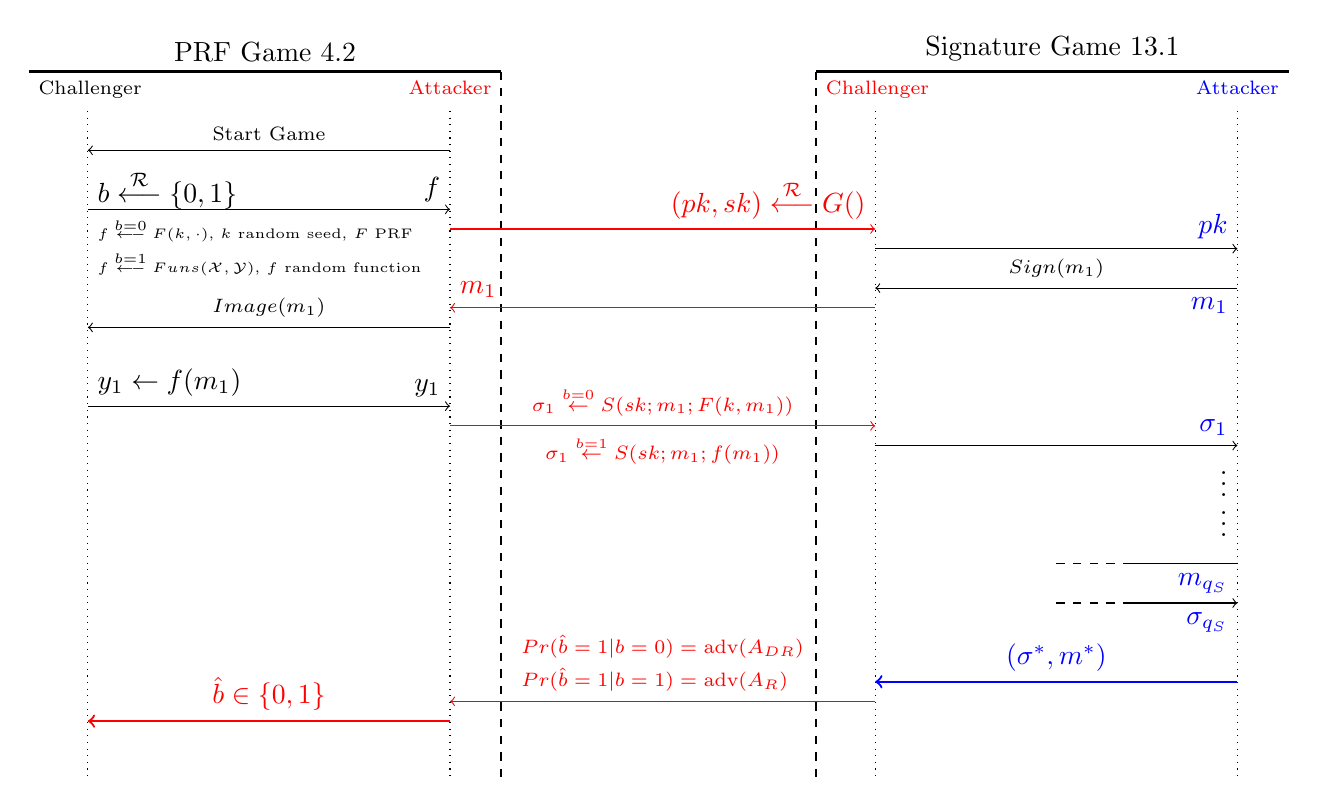
\begin{tikzpicture}
        % Define Variables
        \def\lR{0.75}
        \def\rR{5.35}
        \def\lDR{10.75}
        \def\rDR{15.35}
        \def\bottom{-9}

        % Overall Scheme
        \draw[thick] (0,0) -- (6,0) node[midway, anchor=south] {PRF Game $4.2$};
        \node[anchor = north west] at (0,0) (c-r) {\scriptsize Challenger};
        \draw[dotted] (\lR, -0.5) -- (\lR,\bottom);
        \node[anchor = north east, text=red] at (6,0) {\scriptsize Attacker};
        \draw[dotted] (\rR, -0.5) -- (\rR, \bottom);
        \draw[thick, dashed] (6,0) -- (6, \bottom);
        \draw[thick] (10,0) -- (16,0) node[midway, anchor=south] {Signature Game $13.1$};
        \node[anchor = north west, text=red] at (10,0) {\scriptsize Challenger};
        \node[anchor = north east, text=blue] at (16,0) {\scriptsize Attacker};
        \draw[thick, dashed] (10,0) -- (10, \bottom);
        \draw[dotted] (\lDR, -0.5) -- (\lDR, \bottom);
        \draw[dotted] (\rDR, -0.5) -- (\rDR, \bottom);

        % Start Games
        \draw[->] (\rR, -1) -- (\lR, -1) node[midway, anchor=south] {\scriptsize Start Game};
        \draw[->] (\lR, -1.75) -- (\rR, -1.75) node[midway, anchor=south] {};
        \node[anchor=west] at (\lR, -1.5) {$b \overset{\mathcal{R}}{\longleftarrow} \{0,1\}$};
        \node[anchor=north west, align=left] at (\lR, -1.75) {\tiny $f \overset{b=0}{\longleftarrow} F(k, \cdot)$, $k$ random seed, $F$ PRF \\ \tiny $f \overset{b=1}{\longleftarrow} Funs(\mathcal{X}, \mathcal{Y})$, $f$ random function};
        \node[anchor=east] at (\rR, -1.5) {$f$};
        \node[anchor=south east, color=red] at (\lDR, -2) {$(pk, sk) \overset{\mathcal{R}}{\longleftarrow} G()$};
        \draw[->,color=red] (\rR, -2) -- (\lDR, -2);
        \draw[->] (\lDR, -2.25) -- (\rDR, -2.25) node[anchor=south east, text=blue] {$pk$};

        % First Signing Query
        \draw[->] (\rDR, -2.75) -- (\lDR, -2.75) node[midway, anchor=south] {\scriptsize $Sign(m_1)$};
        \node[anchor=north east, text=blue] at (\rDR, -2.75) {$m_1$};
        \draw[->,color=red] (\lDR, -3) -- (\rR, -3) node[text=red,anchor=south west] {$m_1$};
        \draw[->] (\rR, -3.25) -- (\lR, -3.25) node[midway, anchor=south] {\scriptsize $Image(m_1)$};
        \node[anchor=south west] at (\lR, -4.25) {$y_1 \leftarrow f(m_1)$};
        \draw[->] (\lR, -4.25) -- (\rR, -4.25) node[anchor=south east] {$y_1$};
        \draw[->,color=red] (\rR, -4.5) -- (\lDR, -4.5) node[midway, anchor=south] {\scriptsize $\sigma_1 \overset{b=0}{\leftarrow} S(sk;m_1;F(k, m_1))$} node[midway, anchor=north] {\scriptsize $\sigma_1 \overset{b=1}{\leftarrow} S(sk;m_1;f(m_1))$};
        \draw[->] (\lDR, -4.75) -- (\rDR, -4.75) node[anchor=south east, text=blue] {$\sigma_1$};

        % Next Signing Queries
        \node[anchor=north east] at (\rDR, -4.75) {$\vdots$};
        \node[anchor=north east] at (\rDR, -5.25) {$\vdots$};
        \draw (\rDR, -6.25) node[anchor=north east, text=blue] {$m_{q_S}$} -- (14, -6.25);
        \draw[dashed] (14, -6.25) -- (13, -6.25);
        \draw[dashed] (14, -6.75) -- (13, -6.75);
        \draw[->] (14, -6.75) -- (\rDR, -6.75) node[anchor=north east, text=blue] {$\sigma_{q_S}$};

        % Forgery
        \draw[->, thick, color=blue] (\rDR, -7.75) -- (\lDR, -7.75) node[midway, anchor=south] {$(\sigma^*, m^*)$};
        \draw[->, thick, color=red] (\rR, -8.25) -- (\lR, -8.25) node[midway, anchor=south] {$\hat{b} \in \{0,1\}$};
        \draw[->, color=red] (\lDR, -8) -- (\rR, -8) node[midway, anchor=south, text=red, align=left] {\scriptsize $Pr(\hat{b} = 1 | b = 0) = \text{adv}(A_{DR})$ \\ \scriptsize $Pr(\hat{b} = 1 | b = 1) = \text{adv}(A_{R})$};
        

    \end{tikzpicture}
    \caption{Attack to the $PRF$ game triggering an attacker for the Signature one. In red are the two roles that we actively play, and in black and blue two different entities respectively.\label{fig:attack-game}}
\end{figure}

Initially, the challenger in the $PRF$ game randomly chooses $b = 0,1$:
\begin{itemize}
    \item If $b = 0$: he picks $k \overset{R}{\longleftarrow} \mathcal{K}$ and $f \leftarrow F(k, \cdot)$ a PRF.
    \item If $b = 1$: he picks a random function $f$, that effectively given an input returns a random output.
\end{itemize}
Once we, the attacker in $PRF$, receive $f$, we call the generating algorithm $(pk, sk) \leftarrow G()$ and initialize the Signature Game by sending $pk$ to the attacker in the signature game.

For each signing query $Sign(m_i)$ we receive from the attacker, we forward $m_i$ to the challenger in $PRF$ and receive $f(m_i)$.
We then respond to the signing query with $\sigma_i \leftarrow S(sk, m_i; f(m_i))$.
Observe that:
\begin{itemize}
    \item If $b = 0$: $\sigma_i \leftarrow S(sk, m_i; F(k, m_i))$ for $F$ PRF and $k$ a random seed. Hence effectively playing the game for $S_{DR}$.
    \item If $b = 1$: $\sigma_i \leftarrow S(sk, m_i; r_i)$ for a random $r_i$. Hence effectively playing the game for $S_R$.
\end{itemize}

Once the attacker for $S$ has performed all of its signing queries, he will output a forgery candidate $(\sigma^*, m^*)$.
We will output $1$ in the $PRF$ game if the forgery is valid.
For $b = 0,1$, let $W_b$ be the event that we output $1$ in the PRF game given the value of $b$. Then,
\begin{equation*}
    \begin{split}
        Pr(W_0) &= Pr(A_{PRF} = 1 | b = 0) = Pr((\sigma^*, m^*) \text{ is a valid forgery} | b = 0) = \text{adv}(S_{DR}) \\
        Pr(W_1) &= Pr(A_{PRF} = 1 | b = 1) = Pr((\sigma^*, m^*) \text{ is a valid forgery} | b = 1) = \text{adv}(S_{R}) \\
    \end{split}
\end{equation*}
where the probability of breaking the signature game is also denoted as the advantage.

Lastly, in Definition 4.21, we define the advantage in the $PRF$ game as:
\begin{equation*}
    \begin{split}
        \text{adv}(PRF) &= Pr(W_0) - Pr(W_1) = \text{adv}(S_{DR}) - \text{adv}(S_R) \Leftrightarrow \\
        \text{adv}(S_{DR}) &= \text{adv}(PRF) + \text{adv}(S_R) \leq \varepsilon_{PRF} + \varepsilon_{R}
    \end{split}
\end{equation*}
where we have used that, as $F$ was $PRF$ secure by hypothesis and so was $S$, the advantages in these games are neglegible, hence the advantage for $S_{DR}$ is also neglegible, and the signature scheme secure as we wanted to prove. \hfill $\qed$

\newpage
\section{Problem 4: Secret Sharing Schemes}\label{sec:problem4}

Let $p$ be a prime and let $q = p^r$ for some positive integer $r\in \Z ^+$.
Let $\P$ be a set of participants and $\Gamma \subset 2^\P$ be a monotone increasing access structure.

\begin{enumerate}
    \item Prove that if $\Gamma$ admits a vector space secret sharing scheme over $\F_p$, then $\Gamma$ admits a vector space secret sharing scheme over $GF(q)$.
    \item To prove that the opposite implication is not true, consider the threshold access structure for $n=4$ and $t=2$. Show that this access structure cannot admit a vector space secret sharing scheme over $F_2$, but it admits a vector space secret sharing scheme (which one?) over $GF(2^3)$.
\end{enumerate}

\begin{center}
    \rule{5cm}{0.4pt}
\end{center}

\textbf{\textit{Proof (1):}}
Since $\Gamma$ admits a vector space secret sharing scheme over $\F_p$, there exist $m\in \Z^+$ and $\psi : \P\cup \{D\} \to \F_p^m$ such that $A\in \Gamma$ if and only if $\psi(D)\in\langle \{\psi(P_j)\}_{P_j\in A}\rangle$.
Define
\begin{equation*}
    \begin{split}
        \Psi: \P\cup\{D\} &\longrightarrow (\F_p^m)^r\\
        P &\longmapsto (\psi(P),\ldots, \psi(P)).
    \end{split}
\end{equation*}
Suppose that we want to share a secret $S = (s_1, \ldots, s_r) \in GF(q)$.
Choose a random vector $v = (v_1, \ldots, v_r)\in (\F_p^m)^r$ satisfying $$v \cdot \Psi(D) = (v_1 \cdot \psi(D), \ldots, v_r \cdot \psi(D)) = (s_1, \ldots, s_r) = S,$$ and for $j = 1,\ldots, n$, let $S_j = v\cdot\Psi(P_j)$ be the piece of secret that each $P_j$ can compute.

If $A\in \Gamma$, by hypothesis we have that 
\begin{equation*}
    \begin{split}
        \psi(D) = \sum_{P_j\in A} \lambda^A_j \psi(P_j) \Rightarrow \Psi(D) = \sum_{P_j\in A} \lambda^A_j \Psi(P_j).
    \end{split}
\end{equation*}
Hence, the secret we wanted to share can be recovered by a linear combination of the pieces computed by the participants in $A$, 
\begin{equation*}
    \begin{split}
        \sum_{P_j \in A} \lambda^A_j S_j = \sum_{P_j \in A} \lambda^A_j v\cdot \Psi(P_j) = v\cdot (\sum_{P_j \in A} \lambda^A_j \Psi(P_j)) = v\cdot \Psi(D) = S.
    \end{split}
\end{equation*}

Observe that $(\F_p^m)^r \cong GF(q)^m$ because two finite fields of the same cardinality are isomorphic.
Via this isomorphism, it is clear that we can redefine $\Psi$ to have image in $GF(q)^m$.
Also, the coefficients $\lambda^A_j$ can be embedded in $GF(q)$ using the natural inclusion.

If $B\not \in \Gamma$, we want to see that the shares of participants in $B$ do not give any information about the secret.
The vector space secret sharing scheme over $\F_p$ satisfies that the probability of obtaining the pieces of the participants in $B$ is the same for any secret in $\F_p$.
Then, since $\psi(D) \not \in \langle \{\psi(P_j)\}_{P_j\in B}\rangle$ and by construction of $\Psi$, any possible secret in $GF(q)$ is also equally likely from the shares $\{S_j\}_{P_j\in B}$. 

Therefore, $\Gamma$ admits a vector space secret sharing scheme over $GF(q)$. \hfill $\qed$

\begin{center}
    \rule{5cm}{0.4pt}
\end{center}

\textbf{\textit{Proof (2):}}
Suppose that the $(2,4)$-threshold access structure, $\P = \{P_1, P_2, P_3, P_4\}$ and $\Gamma = \binom{\P}{2}$,  admits a vector space secret sharing scheme ove $\F_2$.
Let $\psi: \P \to \F_2^m$ be a map such that $A\in\Gamma$ if and only if $\psi(D)\in\langle \{\psi(P_j)\}_{P_j\in A}\rangle$, with $\psi(D) \in \F_2^m\setminus\{0\}$.
In particular, $\psi$ must satisfy
\begin{equation*}
    \begin{split}
        \psi(D) = & \lambda_1\psi(P_1) + \lambda_2\psi(P_2)\\
        \psi(D) = & \lambda_3\psi(P_2) + \lambda_4\psi(P_3)\\
        \psi(D) = & \lambda_5\psi(P_1) + \lambda_6\psi(P_3)
    \end{split}
\end{equation*}
for some $\lambda_i \in \F_2$.
In fact, $\lambda_i = 1 \forall i$ because a minimum of two participants is needed to recover the secret.
If we sum the first two equations, we get the contradiction $$0 = \psi(D) + \psi(D) = \psi(P_1) + \psi(P_3) = \psi(D).$$
Hence, the $(2,4)$-threshold access structure does not admit a vector space secret sharing scheme over $\F_2$.

To end, let us construct a vector space secret sharing scheme over $GF(8)$, as a counterexample of the opposite implication of the statement in (1).
First of all, recall that $GF(8)$ is the field of polynomials in $\F_2[x]$ of degree less than 3.
Define $\Psi : \P\cup\{D\} \to GF(8)^2$ by $\Psi(D) = (1, 0), \Psi(P_1) = (1, x), \Psi(P_2) = (1, x+1), \Psi(P_3) = (1, x^2), \Psi(P_4) = (1, x^2+1)$.
To satisfy the condition $A\in\Gamma$ if and only if $\Psi(D)\in\langle \{\Psi(P_j)_{P_j\in A}\}\rangle$, we have to solve
\begin{equation*}
    \begin{split}
        \Psi(D) = \lambda_{ij}\Psi(P_i) + \mu_{ij}\Psi(P_j), \text{ for } i < j.
    \end{split}
\end{equation*}
Let us compute the solution for our choice of $\Psi$:
\begin{equation*}
    \begin{split}
        \left.\begin{aligned}
        1 & = \lambda_{12} + \mu_{12}\\
        0 & = \lambda_{12} x + \mu_{12} (x+1)\\
        \end{aligned}\right\} & \iff \lambda_{12} = x + 1, \mu_{12} = x,\\
        \left.\begin{aligned}
        1 & = \lambda_{13} + \mu_{13}\\
        0 & = \lambda_{13} x + \mu_{13} x^2\\
        \end{aligned}\right\} & \iff \lambda_{13} = x^2+x+1,\mu_{13} = x^2+x,\\
        \left.\begin{aligned}
        1 & = \lambda_{14} + \mu_{14}\\
        0 & = \lambda_{14} x + \mu_{14} (x^2+1)\\
        \end{aligned}\right\} & \iff \lambda_{14} = x,\mu_{14} = x+1,\\
        \left.\begin{aligned}
        1 & = \lambda_{23} + \mu_{23}\\
        0 & = \lambda_{23} (x+1) + \mu_{23} x^2\\
        \end{aligned}\right\} & \iff \lambda_{23} = x^2+x,\mu_{23} = x^2+x+1,\\
        \left.\begin{aligned}
        1 & = \lambda_{24} + \mu_{24}\\
        0 & = \lambda_{24} (x+1) + \mu_{24} (x^2+1)\\
        \end{aligned}\right\} & \iff \lambda_{24} = x^2,\mu_{24} = x^2+1,\\
        \left.\begin{aligned}
        1 & = \lambda_{34} + \mu_{34}\\
        0 & = \lambda_{34} x^2 + \mu_{34} (x^2+1)\\
        \end{aligned}\right\} & \iff \lambda_{34} = x^2+1,\mu_{34} = x^2.\\
    \end{split}
\end{equation*}
To share a secret $s \in GF(8)$, we have to choose a random vector $v\in GF(8)^2$ such that $v\cdot\Psi(D) = s$.
Each participant $P_j$ is able to compute $s_j = v\cdot \Psi(P_j)$, and the secret can be recovered using the computed coefficients, 
\begin{equation*}
    \begin{split}
        s = \lambda_{ij}s_i + \mu_{ij}s_j,
    \end{split}
\end{equation*}
for each pair $(i,j)$ with $i<j$.
Observe that only one participant does not give any information about the secret.

This vector space secret sharing scheme is the well-known Shamir secret sharing scheme.
For a general $(t, n)$-threshold access structure and a finite field $\F$ with more than $n$ elements, we have to choose $n$ different elements $\alpha_1,\ldots,\alpha_n \in \F\setminus\{0\}$, and define $\Psi(D) = (1,0, \ldots, 0)$, $\Psi(P_i) = (1, \alpha_i, \ldots, \alpha_i^{t-1})$. \hfill $\qed$



\end{document}
